% !TeX root = ../../main.tex
\subsection{Longitudinal Cas13 reanalysis separates ranking from calibration}
\label{sec:liang}

The Cas13 fitness screens of \citet{liang2026lncrna} provide a stringent test
of whether the CB\textsuperscript{2} sampling model can support a genuinely
longitudinal design.  We analysed all deposited measurements from days 0, 7,
and 14 in five cell lines.  BARCS, MAGeCK-MLE, edgeR-QL, DESeq2, and
limma--voom estimated the same continuous time slope.  Replicate was included
when complete trajectories were available; K562 lacked one day-0 replicate
and was fitted without the replicate block.  The longitudinal regression
methods used two-sided significance tests.

The deposited values had already undergone median-of-ratios normalization,
ComBat correction, and replicate-outlier processing.  We rounded them once to
the nearest pseudo-count and supplied the same matrix to every method.
Accordingly, this is a processed-count sensitivity analysis rather than a
raw-count likelihood comparison.

Using the intermediate day improved BARCS average precision from 0.776 to
0.786 and recall at gene FDR 0.10 from 0.487 to 0.580 relative to the
two-endpoint fit.  Against longitudinal MAGeCK-MLE, BARCS substantially
improved null calibration: mean absolute calibration error was 0.035 versus
0.103, with average precision 0.786 versus 0.833.  The three general RNA-seq
models had mean null $p<0.05$ rates of 0.139--0.153, compared with 0.076 for
BARCS.

The paired cell-line comparison shows why this difference matters.  BARCS had
the lowest mean absolute calibration error, 0.035, compared with
0.093--0.107 for the alternative longitudinal regression models, while
essential-gene recall at the same empirical 5\% null false-positive rate
remained comparable (0.820 versus 0.840--0.853).  The largest calibration
gains occurred in K562 and MDA-MB-231, where the alternative null rates were
22.4--33.9\% and 14.0--20.0\%, respectively.
Figure~\ref{fig:liang} first shows the complete longitudinal volcano plot for
each method across all five cell lines.  Panels A--C then show three
prespecified-null guide examples for which calibrated BARCS returned
$p=0.20$--$0.23$, while DESeq2, edgeR-QL, and limma--voom each returned
$p<0.05$.  Their library-normalized guide-count trajectories retain both
replicates at each available day, making the longitudinal evidence directly
visible.  These are false-positive calls under the benchmark's prespecified
null definition, not additional biological discoveries.

\begin{figure}[htbp]
\centering
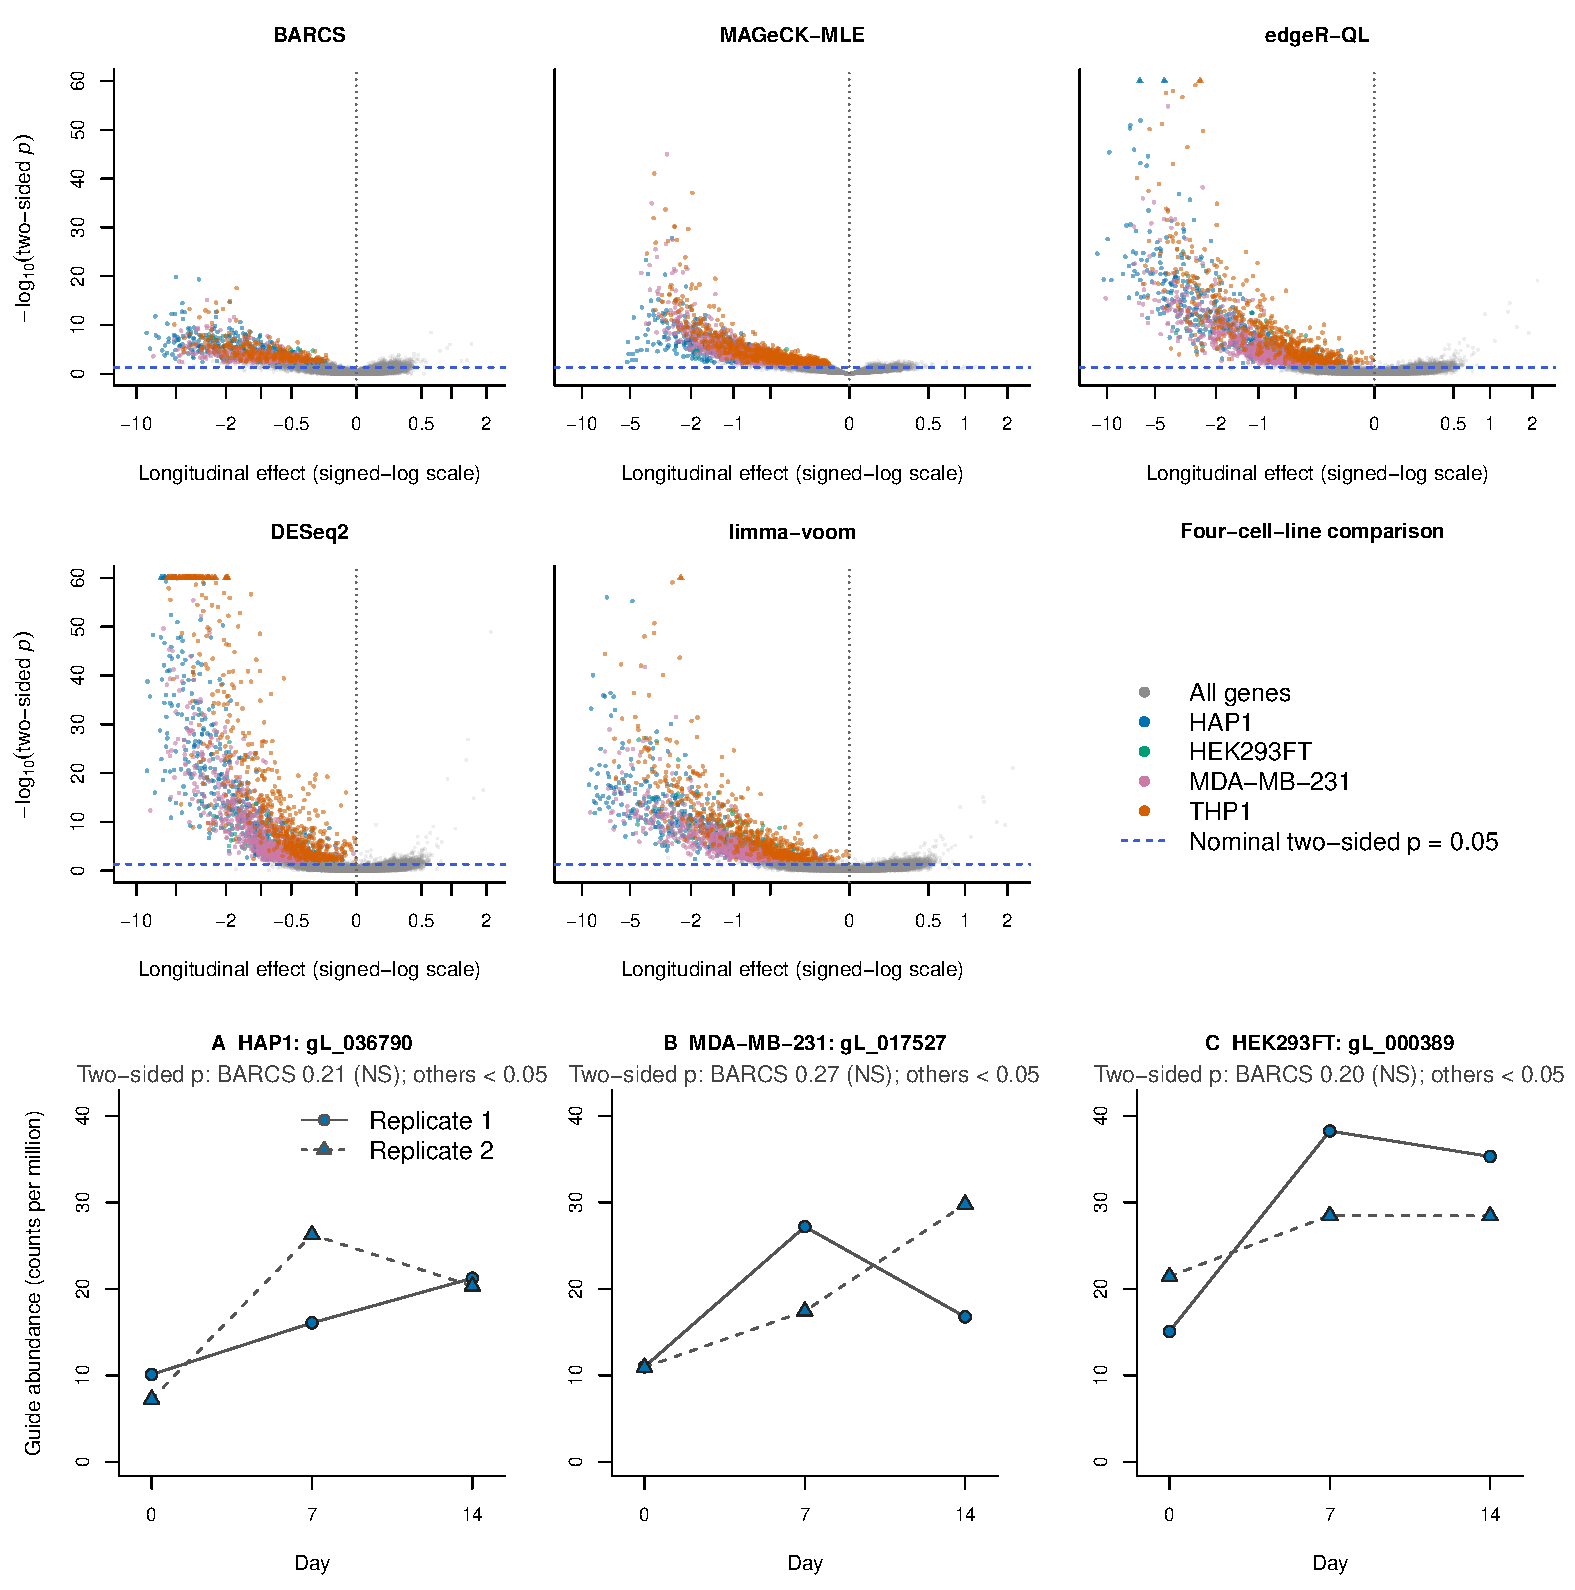
\includegraphics[width=\textwidth]{figures/liang_longitudinal_volcano_trajectories.pdf}
\caption{Longitudinal Cas13 comparison using days 0, 7, and 14.  The upper
rows show method-specific volcano plots for BARCS, MAGeCK-MLE, edgeR-QL,
DESeq2, and limma--voom, pooling gene-level results from HAP1, HEK293FT, K562,
MDA-MB-231, and THP1.  Within each cell line, every method estimates the same
continuous time slope from the identical processed-count matrix.  Colored
points are negatively directed genes called at two-sided FDR 0.10, with color
denoting cell line; the dashed horizontal line marks nominal two-sided
$p=0.05$, and triangles identify $-\log_{10}(p)$ values clipped at 60.
(A--C) Processed
guide counts divided by the corresponding library size, in counts per
million, for three prespecified-null examples.  Lines connect measurements
from the same replicate across days.  BARCS leaves each guide non-significant,
whereas DESeq2, edgeR-QL, and limma--voom each call it significant.
MAGeCK-MLE is included in the gene-level volcano comparison but not in panels
A--C because its reported statistic is gene-level.}
\label{fig:liang}
\end{figure}

Rounding changed each deposited value by less than 0.5, but the upstream
transformations mean that none of the fitted likelihoods retains its literal
raw-count interpretation.  Confirmation from raw reads therefore remains
necessary.  The supplied streaming workflow performs the full longitudinal
preparation for that validation.
